\documentclass[11pt]{article}

\usepackage[margin=1in]{geometry}
\usepackage[T1]{fontenc}
\usepackage{lmodern}
\usepackage{microtype}
\usepackage{amsmath,amssymb}
\usepackage{booktabs}
\usepackage{graphicx}
\usepackage{float}
\usepackage[font=small,labelfont=bf]{caption}
\usepackage{verbatim}
\usepackage[hidelinks]{hyperref}

\newcommand{\sm}{\texttt{statsmodels}}
\newcommand{\st}{ScalaTion}
\newcommand{\bb}{\boldsymbol{\beta}}

\title{Ridge and Lasso Regression on AutoMPG\\[2pt]
\large ScalaTion and \texttt{statsmodels}}
\author{CSCI 4360 Data Science ML II}
\date{\today}

\begin{document}
\maketitle

\begin{abstract}
\noindent We fit Ridge and Lasso to the AutoMPG data in ScalaTion and in \texttt{statsmodels}. Each package also gets a
plain least squares (OLS) fit to compare against. Both packages use the same train/test split, the same
cross-validation folds, the same scaling and the same list of penalty values. Ridge gives the same coefficients in both
packages (they match to about $10^{-8}$). Lasso differs by at most $0.07$ because ScalaTion only solves it approximately.
All six models have a test RMSE between $3.23$ and $3.28$~mpg, and the two Lasso models are the best of the six. Weight and
model year explain almost all of the fuel economy.
\end{abstract}

\section{Data}

We used the UCI Auto MPG data \cite{quinlan1993}. The response is fuel economy in miles per gallon (\texttt{mpg}). The six
predictors are \texttt{cylinders}, \texttt{displacement}, \texttt{horsepower}, \texttt{weight}, \texttt{acceleration} and
\texttt{model\_year}. Six cars have no \texttt{horsepower}, so we dropped them and kept $392$ rows. We left out the
\texttt{origin} column, as ScalaTion's own \texttt{Example\_AutoMPG} does, because it is a category code that can overlap
with the other predictors. The ScalaTion run uses ScalaTion's built-in copy of the data. The program checks that its totals match the UCI file
($\sum\texttt{mpg}=9190.8$, $\sum\texttt{weight}=1\,167\,213$), and the ScalaTion OLS fit matches the \texttt{statsmodels} OLS
fit to $10^{-8}$, so the rows and their order are the same.

\begin{table}[htbp]
\centering\small
\begin{tabular}{@{}lrrrrr@{}}
\toprule
Variable & Mean & Std.\ dev. & Min & Max & VIF \\
\midrule
mpg (response) & 23.45 & 7.81 & 9.0 & 46.6 & n/a \\
cylinders & 5.47 & 1.71 & 3.0 & 8.0 & 10.99 \\
displacement & 194.41 & 104.64 & 68.0 & 455.0 & 19.30 \\
horsepower & 104.47 & 38.49 & 46.0 & 230.0 & 9.39 \\
weight & 2977.58 & 849.40 & 1613.0 & 5140.0 & 10.06 \\
acceleration & 15.54 & 2.76 & 8.0 & 24.8 & 2.68 \\
model\_year & 75.98 & 3.68 & 70.0 & 82.0 & 1.27 \\
\bottomrule
\end{tabular}
\caption{The 392 cars. VIF (variance inflation factor) is computed on the 314 training rows.}\label{tab:data}
\end{table}

Table~\ref{tab:data} shows that the engine-size variables move together. The VIFs of \texttt{displacement},
\texttt{cylinders}, \texttt{weight} and \texttt{horsepower} are all about $9$ or higher, and \texttt{cylinders} and
\texttt{displacement} have a correlation of $0.95$. In this situation the OLS coefficients are unstable even though the model
predicts well. Ridge and Lasso are meant for this.

\section{Method}

\paragraph{Split and folds.} We split the $392$ rows into $314$ training rows and $78$ test rows (seed $42$). We picked the
penalty using only the training rows, with $5$-fold cross-validation. The Python script saves the test rows and the fold of
every training row to \texttt{data/test\_indices.csv} and \texttt{data/cv\_folds.csv}. The ScalaTion program reads the same
files, so both packages see the same data at every step.

\paragraph{Scaling.} Each predictor is scaled to mean $0$ and standard deviation $1$, using the training rows only (inside
each CV fold, using only that fold's training rows). The intercept is never penalized. Coefficients are therefore in
``mpg per one standard deviation of the predictor''. Table~\ref{tab:coef-orig} gives them in the original units too.

\paragraph{Penalties.} With $n$ training rows, scaled predictors $\mathbf z_i$ and intercept $\beta_0$, ScalaTion minimizes
\begin{align*}
\text{Ridge:}\quad & \sum_i (y_i-\beta_0-\mathbf z_i^\top\bb)^2+\lambda\|\bb\|_2^2,\\
\text{Lasso:}\quad & \tfrac12\sum_i (y_i-\beta_0-\mathbf z_i^\top\bb)^2+\lambda\|\bb\|_1 .
\end{align*}
\texttt{statsmodels} minimizes $\frac{1}{2n}\mathrm{RSS}+\alpha\big[\tfrac{1-w}{2}\|\bb\|_2^2+w\|\bb\|_1\big]$, with $w=0$ for Ridge
and $w=1$ for Lasso. Multiply by $n$ and the two forms are the same when
\[
\lambda = n\,\alpha \qquad\text{(Ridge and Lasso)}.
\]
We report every penalty as $\lambda=n_{\text{train}}\alpha$ with $n_{\text{train}}=314$.

\paragraph{Tuning.} Both packages try the same $60$ values of $\alpha$, spaced evenly on a log scale from $10^{-4}$ to $10$
(so $\lambda$ runs from $0.031$ to $3140$). We keep the value with the lowest $5$-fold CV RMSE. The same list of values gives
the coefficient paths.

\paragraph{\texttt{statsmodels}.} We used \texttt{sm.OLS(...).fit\_regularized(method="elastic\_net")} (version 0.15.0). Two
things needed care. First, it shrinks every column, including the intercept, unless you give a separate penalty for each
coefficient. With one penalty value, the Ridge intercept dropped from $23.4$ to $15.6$ in a quick test. We give the intercept a penalty
of $0$. Second, the Lasso solver never looks at a coefficient again once it reaches zero (the source code says this), so one
call can stop too early. We run it again from its last answer until nothing changes. The unit tests check the result against
scikit-learn's Lasso and against the optimality conditions (Section~\ref{sec:tests}).

\paragraph{ScalaTion.} We used \texttt{RidgeRegression.rescale} and \texttt{LassoRegression.rescale}. They scale $X$ with
\texttt{NormForm} and center $y$, so the intercept is the training mean of \texttt{mpg} and is not penalized. Ridge is solved
directly (Cholesky). Lasso is solved with ADMM (\texttt{LassoAdmm}). The two classes share one hyper-parameter object, so the program
sets $\lambda$ right before it builds each model and clears the ADMM warm-start cache before each Lasso fit. The OLS fit is
ScalaTion's \texttt{Regression} on $[\mathbf 1,\mathbf Z]$. We wrote the cross-validation loop ourselves (fit on four folds,
predict the fifth) instead of using ScalaTion's \texttt{findLambda}, because \texttt{findLambda} only doubles $\lambda$ from a start
value and cannot use our list of values or our folds.

\paragraph{Metrics.} RMSE, $R^2$ and MAE on the $314$ training rows and on the $78$ test rows, plus the $5$-fold CV RMSE (the
square root of the mean fold MSE).

\section{Results}

\subsection{Overview}

Table~\ref{tab:summary} lists all six models. Figure~\ref{fig:cv} shows the CV curves, Table~\ref{tab:coef-std} the
coefficients, and Figures~\ref{fig:paths} and~\ref{fig:zoom} the coefficient paths.

\begin{table}[htbp]
\centering\small
\resizebox{\textwidth}{!}{\begin{tabular}{@{}llrrrrrrr@{}}
\toprule
Software & Model & $\lambda$ & Zero coef. & CV RMSE & Train $R^2$ & Test $R^2$ & Test RMSE & Test MAE \\
\midrule
statsmodels & OLS & n/a & 0/6 & 3.5852 & 0.8105 & 0.7945 & 3.2526 & 2.5068 \\
statsmodels & Ridge & 5.02 & 0/6 & 3.5747 & 0.8097 & 0.7914 & 3.2769 & 2.5190 \\
statsmodels & Lasso & 19.66 & 1/6 & 3.5414 & 0.8104 & 0.7960 & 3.2404 & 2.4870 \\
\midrule
ScalaTion & OLS & n/a & 0/6 & 3.5852 & 0.8105 & 0.7945 & 3.2526 & 2.5068 \\
ScalaTion & Ridge & 3.39 & 0/6 & 3.5747 & 0.8101 & 0.7923 & 3.2700 & 2.5137 \\
ScalaTion & Lasso & 29.04 & 0/6 & 3.5387 & 0.8103 & 0.7969 & 3.2332 & 2.4773 \\
\bottomrule
\end{tabular}}
\caption{Fit and prediction results. $\lambda=n_{\text{train}}\alpha$ is the penalty picked by 5-fold CV. ``Zero coef.''
counts slopes that are exactly zero (out of $6$). Test columns use the $78$ test cars. CV RMSE uses the $314$ training cars.}\label{tab:summary}
\end{table}

\begin{table}[htbp]
\centering\small
\begin{tabular}{@{}lrrrrrr@{}}
\toprule
 & \multicolumn{3}{c}{statsmodels} & \multicolumn{3}{c}{ScalaTion} \\
\cmidrule(lr){2-4}\cmidrule(lr){5-7}
Term & OLS & Ridge & Lasso & OLS & Ridge & Lasso \\
\midrule
intercept & 23.6102 & 23.6102 & 23.6102 & 23.6102 & 23.6102 & 23.6102 \\
cylinders & $-$0.1931 & $-$0.2752 & $-$0.1509 & $-$0.1931 & $-$0.2434 & $-$0.1485 \\
displacement & 0.0810 & $-$0.3515 & 0.0000 & 0.0810 & $-$0.2421 & $-$0.0030 \\
horsepower & $-$0.0874 & $-$0.4120 & $-$0.1671 & $-$0.0874 & $-$0.3243 & $-$0.2048 \\
weight & $-$5.5169 & $-$4.7868 & $-$5.3947 & $-$5.5169 & $-$4.9876 & $-$5.3513 \\
acceleration & 0.1663 & $-$0.0098 & 0.0902 & 0.1663 & 0.0360 & 0.0597 \\
model\_year & 2.7513 & 2.6577 & 2.7000 & 2.7513 & 2.6849 & 2.6764 \\
\bottomrule
\end{tabular}
\caption{Coefficients on the scaled predictors (mpg per standard deviation of the predictor). The intercept is the training
mean of \texttt{mpg}. OLS is the same in both packages, so the data, split and scaling agree.}\label{tab:coef-std}
\end{table}

\begin{figure}[htbp]
\centering
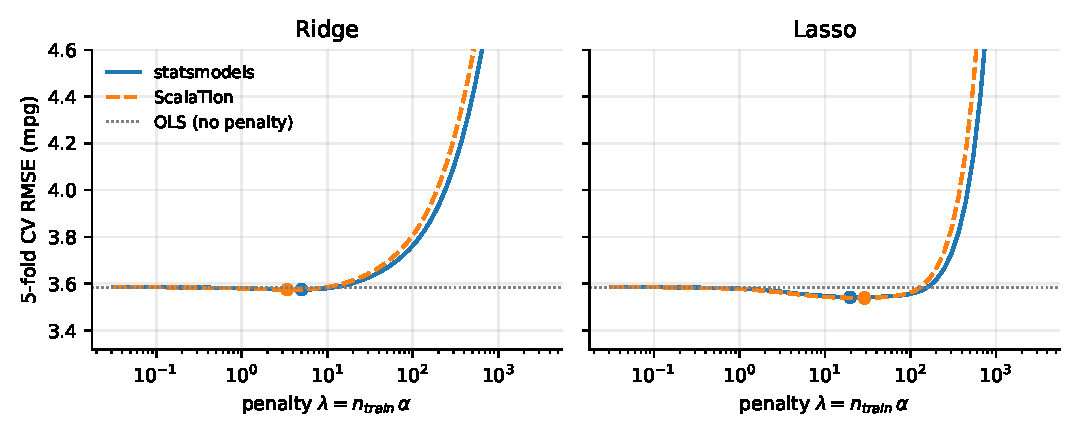
\includegraphics[width=\textwidth]{figures/cv_curves}
\caption{5-fold CV RMSE against the penalty $\lambda=n_{\text{train}}\alpha$. Dots mark the chosen $\lambda$. The Ridge curve
is almost flat up to $\lambda\approx10$. The Lasso curve has a shallow low point near $\lambda\approx20$ to $30$.}\label{fig:cv}
\end{figure}

\begin{figure}[htbp]
\centering
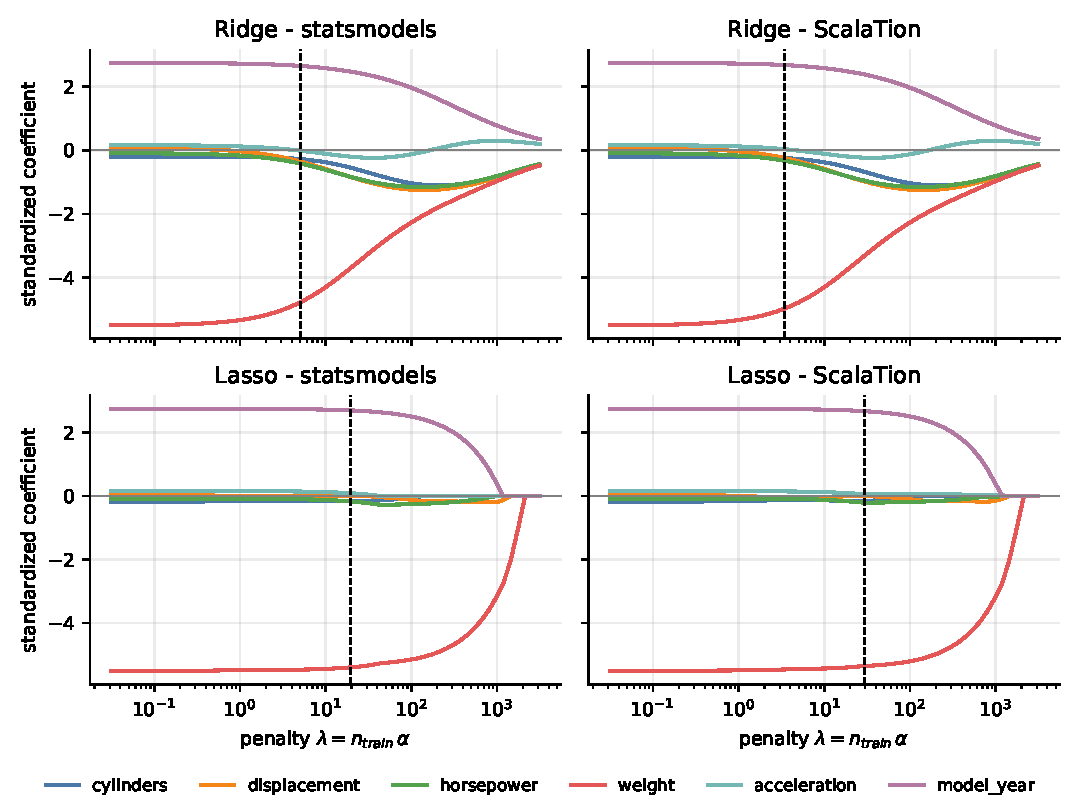
\includegraphics[width=\textwidth]{figures/coefficient_paths}
\caption{Coefficient paths. Dashed lines mark the chosen $\lambda$. Ridge shrinks every coefficient smoothly and none reach zero.
Lasso sets coefficients to zero (\texttt{statsmodels}) or close to zero (ScalaTion).}\label{fig:paths}
\end{figure}

\begin{figure}[htbp]
\centering
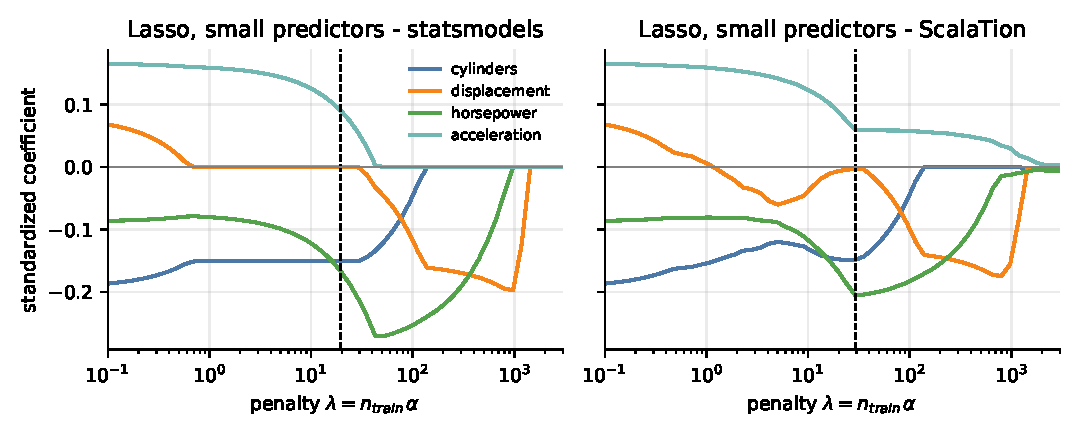
\includegraphics[width=\textwidth]{figures/lasso_zoom}
\caption{Lasso paths for the four small predictors (\texttt{weight} and \texttt{model\_year} left out so the scale is readable).}\label{fig:zoom}
\end{figure}

\subsection{Ridge, \texttt{statsmodels}}\label{sec:ridge-sm}
CV picks $\lambda=5.02$ ($\alpha=0.0160$). Ridge keeps all six predictors. The \texttt{weight} coefficient gets smaller, from
$-5.52$ in OLS to $-4.79$. The three engine-size variables are small and mixed in sign in OLS $(-0.19,+0.08,-0.09)$. Ridge turns
them into a steady negative group $(-0.28,-0.35,-0.41)$ for \texttt{cylinders}, \texttt{displacement} and \texttt{horsepower}. So
Ridge spreads the effect of a bigger engine over the related variables, instead of letting one coefficient take all of it.
\texttt{acceleration} shrinks to about zero ($-0.01$) and \texttt{model\_year} barely changes ($2.75\to2.66$). The predictions are
about the same as OLS: CV RMSE $3.5747$ against $3.5852$, test RMSE $3.277$ against $3.253$, test $R^2$ $0.791$ against
$0.794$. With $314$ rows and six predictors, Ridge does not cut the error much. What it gives us is more believable coefficients, not better predictions.

\subsection{Lasso, \texttt{statsmodels}}\label{sec:lasso-sm}
CV picks $\lambda=19.66$ ($\alpha=0.0626$). \texttt{displacement} is set exactly to zero. The other five stay but shrink:
$\texttt{weight}=-5.39$ (OLS $-5.52$), $\texttt{model\_year}=2.70$, $\texttt{horsepower}=-0.17$,
$\texttt{cylinders}=-0.15$, $\texttt{acceleration}=0.09$. Displacement is probably dropped because it overlaps the most with the
others (VIF $19.3$, correlation $0.95$ with \texttt{cylinders}), so \texttt{cylinders}, \texttt{horsepower} and \texttt{weight}
already carry what it knows. This is the best \texttt{statsmodels} model: CV RMSE $3.5414$ (OLS $3.5852$), test RMSE $3.240$
(OLS $3.253$), test $R^2$ $0.796$. Lasso beat OLS in all five CV folds (by $0.03$ to $0.11$~mpg). Ridge beat OLS in only three. The gain is
steady but small next to the noise in a 78-row test set. We also refit OLS on the five kept predictors (Table~\ref{tab:refit}).
Only \texttt{weight} ($t=-9.7$) and \texttt{model\_year} ($t=12.4$) are clearly different from zero. \texttt{cylinders},
\texttt{horsepower} and \texttt{acceleration} have $p>0.6$. These $p$-values ignore that the variables were picked, so they look
better than they should. They still fit the paths in Figures~\ref{fig:paths} and~\ref{fig:zoom}. As $\lambda$ grows past the chosen
value, the \texttt{statsmodels} Lasso drops \texttt{acceleration} (at $\lambda\approx50$), \texttt{cylinders} ($\approx130$),
\texttt{horsepower} ($\approx900$), \texttt{model\_year} ($\approx1100$) and \texttt{displacement} ($\approx1300$). \texttt{weight}
is the last one left ($\approx1900$).

\begin{table}[htbp]
\centering\small
\begin{tabular}{@{}lrrrrrr@{}}
\toprule
Term & Coef. & Std.\ err. & $t$ & $p$-value & 95\% CI low & 95\% CI high \\
\midrule
intercept & 23.6102 & 0.1968 & 119.99 & 0.0000 & 23.2230 & 23.9974 \\
cylinders & $-$0.1510 & 0.4730 & $-$0.32 & 0.7498 & $-$1.0817 & 0.7798 \\
horsepower & $-$0.0754 & 0.5900 & $-$0.13 & 0.8984 & $-$1.2363 & 1.0854 \\
weight & $-$5.4915 & 0.5634 & $-$9.75 & 0.0000 & $-$6.6001 & $-$4.3829 \\
acceleration & 0.1628 & 0.3202 & 0.51 & 0.6114 & $-$0.4673 & 0.7930 \\
model\_year & 2.7498 & 0.2219 & 12.39 & 0.0000 & 2.3132 & 3.1865 \\
\bottomrule
\end{tabular}
\caption{\texttt{statsmodels}: plain OLS refit on the predictors Lasso kept (scaled predictors). The $p$-values ignore the selection step.}\label{tab:refit}
\end{table}

\subsection{Ridge, ScalaTion}\label{sec:ridge-st}
CV picks $\lambda=3.39$ ($\alpha=0.0108$), with the same CV RMSE as \texttt{statsmodels} ($3.5747$). The coefficients
$(-0.24,-0.24,-0.32,-4.99,+0.04,+2.68)$ follow the same pattern as in \texttt{statsmodels}: weight shrinks a little, the three
engine-size variables become a steady negative group, and \texttt{acceleration} is close to zero. Test RMSE is $3.270$ and test
$R^2$ is $0.792$, within $0.02$~mpg of OLS ($3.253$). These coefficients differ from the \texttt{statsmodels} Ridge column only
because the two searches landed on different points of an almost flat CV curve ($\lambda=3.39$ against $5.02$, both with CV RMSE $3.5747$).
At the \emph{same} $\lambda$ the two packages agree to $8\times10^{-9}$ along the whole path (Table~\ref{tab:compare}).

\subsection{Lasso, ScalaTion}\label{sec:lasso-st}
CV picks $\lambda=29.04$ ($\alpha=0.0925$). \texttt{displacement} shrinks to $-0.003$. That is zero for practical purposes (under
$0.01$), but ScalaTion does not call it an exact zero (Table~\ref{tab:summary}). Its ADMM solver stops at a loose tolerance, and
its clean-up step only zeroes coefficients below $10^{-3}$ of the largest one ($0.0027$ here). The other coefficients
$(\texttt{cylinders}=-0.15,\ \texttt{horsepower}=-0.20,\ \texttt{weight}=-5.35,\ \texttt{acceleration}=0.06,\
\texttt{model\_year}=2.68)$ tell the same story as \texttt{statsmodels}: weight and model year matter most and the engine-size
variables are small. This is the best of the six models by test error (RMSE $3.233$, $R^2$ $0.797$) and by CV RMSE ($3.5387$).
ScalaTion's own coefficient table for Ridge and Lasso prints standard errors, $t$ values and $p$ values that assume no
penalty, so they are not valid here and we do not use them (the raw output is in Appendix~\ref{app:native}).

\subsection{The two packages compared}

\begin{table}[htbp]
\centering\small
\begin{tabular}{@{}lrrr@{}}
\toprule
Quantity & OLS & Ridge & Lasso \\
\midrule
Max coefficient gap over the whole $\lambda$ grid & n/a & 7.6e-09 & 7.2e-02 \\
Median coefficient gap over the grid & n/a & 6.6e-09 & 2.0e-02 \\
Max coefficient gap, tuned final models & 7.6e-09 & 2.0e-01 & 4.3e-02 \\
Test-RMSE gap, tuned final models & 4.4e-16 & 6.9e-03 & 7.2e-03 \\
\bottomrule
\end{tabular}
\caption{ScalaTion minus \texttt{statsmodels}, in scaled coefficient units. The path rows compare the two packages at the
\emph{same} $\lambda$ on all $60$ grid points. The final-model rows also include the effect of the two searches picking different $\lambda$.}\label{tab:compare}
\end{table}

\begin{itemize}
\item \textbf{OLS and Ridge agree to about $10^{-8}$.} The OLS coefficients differ by $8\times10^{-9}$ and the Ridge paths by
$8\times10^{-9}$. This also confirms the $\lambda=n\alpha$ link and the matching scaling.
\item \textbf{Lasso differs by at most about $0.07$ (median $0.02$).} Our \texttt{statsmodels} code (with restarts) gives the exact
Lasso answer, as the unit tests show. ScalaTion's \texttt{LassoAdmm} has fixed tolerances ($10^{-4}$ absolute, $10^{-2}$ relative)
that user code cannot change, so its answer is approximate. The ScalaTion path in Figure~\ref{fig:zoom} is less smooth than the exact one.
The gap is about $1\%$ of the largest coefficient and changes no conclusion.
\item \textbf{All six models predict about equally well.} Test RMSE runs from $3.233$ to $3.277$, a spread of $1.3\%$. With $78$
test rows, the standard error of an RMSE is roughly $0.26$~mpg, so none of these differences is meaningful. Do not read much into the ranking.
\end{itemize}

\begin{figure}[htbp]
\centering
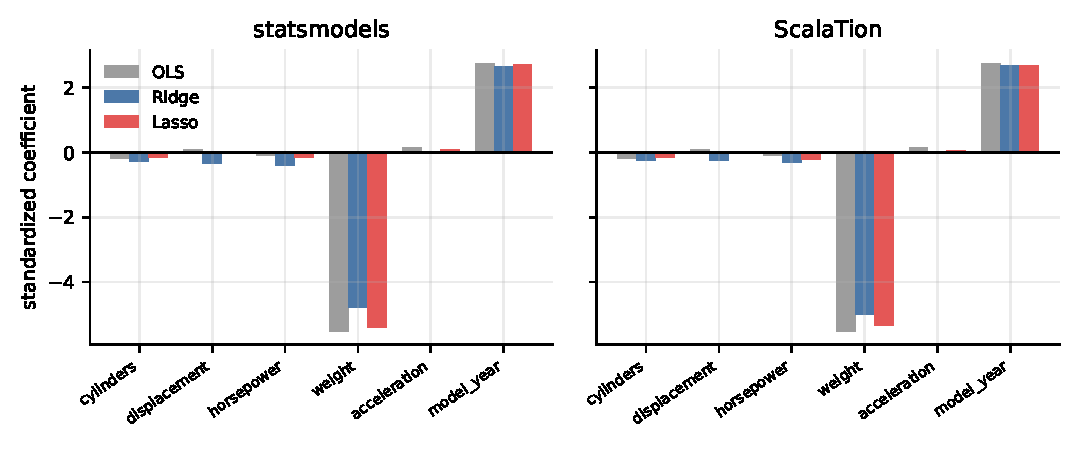
\includegraphics[width=\textwidth]{figures/coefficient_bars}
\caption{Coefficients of the OLS, Ridge and Lasso fits in each package (scaled predictors).}\label{fig:bars}
\end{figure}

\begin{table}[htbp]
\centering\small
\begin{tabular}{@{}lrrrrrr@{}}
\toprule
 & \multicolumn{3}{c}{statsmodels} & \multicolumn{3}{c}{ScalaTion} \\
\cmidrule(lr){2-4}\cmidrule(lr){5-7}
Term & OLS & Ridge & Lasso & OLS & Ridge & Lasso \\
\midrule
intercept & $-$14.59995 & $-$12.29165 & $-$13.30611 & $-$14.59995 & $-$12.95043 & $-$12.69685 \\
cylinders & $-$0.11361 & $-$0.16191 & $-$0.08880 & $-$0.11361 & $-$0.14320 & $-$0.08734 \\
displacement & 0.00078 & $-$0.00339 & 0.00000 & 0.00078 & $-$0.00233 & $-$0.00003 \\
horsepower & $-$0.00229 & $-$0.01077 & $-$0.00437 & $-$0.00229 & $-$0.00848 & $-$0.00536 \\
weight & $-$0.00656 & $-$0.00569 & $-$0.00641 & $-$0.00656 & $-$0.00593 & $-$0.00636 \\
acceleration & 0.05911 & $-$0.00349 & 0.03206 & 0.05911 & 0.01280 & 0.02122 \\
model\_year & 0.75560 & 0.72988 & 0.74152 & 0.75560 & 0.73736 & 0.73503 \\
\bottomrule
\end{tabular}
\caption{The same coefficients in original units, which is mpg per unit of each predictor. For example, the \texttt{statsmodels} Lasso gives
$-0.0064$~mpg per pound (about $-6.4$~mpg per $1000$~lb) and $+0.74$~mpg per model year.}\label{tab:coef-orig}
\end{table}

\subsection{What the fits say about fuel economy}
In every model, heavier cars get lower mpg (about $-4.8$ to $-5.5$ mpg per standard deviation of weight, which is roughly $850$~lb),
and newer model years get higher mpg (about $+2.7$ mpg per standard deviation, roughly $3.7$ years). Once these two are in the model,
cylinders, displacement, horsepower and acceleration add little. They move together with weight, so their own coefficients are small and
change with the penalty. A model with just \texttt{weight} and \texttt{model\_year} already explains most of the variance. The penalty changes how the
credit is split among related predictors much more than it changes the predictions.

\section{Checks}\label{sec:tests}

The Python code has $11$ automatic tests (\texttt{python -m unittest discover -s tests}) and all pass. They check that:
the data has $392$ clean rows and the right \texttt{mpg} total; the split has no overlap, covers every row and gives the same result each time;
scaled columns have mean $0$ and standard deviation $1$; Ridge equals the closed-form answer $(Z^\top Z+n\alpha D)^{-1}Z^\top y$ and
scikit-learn's Ridge with penalty $n\alpha$; Lasso equals scikit-learn's Lasso at $10$ values spread over the grid (within $10^{-6}$)
and meets the optimality (KKT) conditions; the intercept is not penalized; a tiny penalty gives back OLS and a huge Lasso penalty zeroes every
slope; and coefficients converted to original units give the same predictions. The ScalaTion program stops with an error if its data or training rows do not match
the UCI data, and its OLS fit matches the \texttt{statsmodels} OLS fit. ScalaTion's variance inflation factors for the six predictors
($10.99$, $19.30$, $9.39$, $10.06$, $2.68$, $1.27$) match the ones we computed separately in Python (Table~\ref{tab:data}).

\section{Limits}
\begin{itemize}
\item We used one train/test split and one set of CV folds. The CV curves are very flat, so the best $\lambda$ is not well pinned down.
That is why the two packages picked different $\lambda$ values with the same CV RMSE.
\item ScalaTion's built-in \texttt{crossValidate} reuses one scaling for every fold, which lets a little information from the validation rows
leak in. Our own CV loop redoes the scaling inside each fold, in both packages.
\item ScalaTion's Lasso is approximate, so it gives a near-zero value instead of an exact zero for \texttt{displacement}.
\item The $p$-values in Table~\ref{tab:refit} do not account for picking the variables first.
\end{itemize}

\section{How to run}
{\footnotesize\begin{verbatim}
cd Project2/python
pip install -r requirements.txt
python regularized_regression.py     # statsmodels run (also writes the split/fold CSVs)
python -m unittest discover -s tests # 11 tests
# ScalaTion (needs JDK 21 and sbt; Scala 3.8.3): copy
#   scalation/RegularizedRegression_AutoMPG.scala into
#   scalation_2.0/src/main/scala/scalation/modeling/ and run, from scalation_2.0:
#   P2_DIR=<path to Project2> sbt "runMain scalation.modeling.regularizedRegression_AutoMPG"
python compare_results.py            # ScalaTion vs statsmodels
python make_figures.py; python make_tables.py
\end{verbatim}}

\begin{thebibliography}{9}\small
\bibitem{quinlan1993} R.~Quinlan (1993). \emph{Auto MPG}. UCI Machine Learning Repository, \url{https://doi.org/10.24432/C5859H}.
\bibitem{hoerl1970} A.~Hoerl and R.~Kennard (1970). Ridge regression: biased estimation for nonorthogonal problems. \emph{Technometrics} 12(1), 55-67.
\bibitem{tibshirani1996} R.~Tibshirani (1996). Regression shrinkage and selection via the lasso. \emph{J.\ Roy.\ Statist.\ Soc.\ B} 58(1), 267-288.
\bibitem{boyd2011} S.~Boyd et al.\ (2011). Distributed optimization and statistical learning via the alternating direction method of multipliers. \emph{Found.\ Trends Mach.\ Learn.} 3(1), 1-122.
\bibitem{friedman2010} J.~Friedman, T.~Hastie, R.~Tibshirani (2010). Regularization paths for generalized linear models via coordinate descent. \emph{J.\ Stat.\ Softw.} 33(1), 1-22.
\bibitem{seabold2010} S.~Seabold and J.~Perktold (2010). Statsmodels: econometric and statistical modeling with Python. \emph{Proc.\ 9th Python in Science Conf.}
\bibitem{scalation} J.~Miller et al. ScalaTion 2.0, \url{https://github.com/scalation/scalation_2.0}.
\end{thebibliography}

\appendix
\section{ScalaTion output}\label{app:native}
ScalaTion's own fit numbers on the training rows (Table~\ref{tab:native}), then the console listing for each model. The coefficients are on
the scaled predictors. The ``Std.\ Error / $t$ / Pr'' columns use the no-penalty OLS formulas, so they are not valid for Ridge and Lasso.

\begin{table}[htbp]
\centering\small
\begin{tabular}{@{}lrrrrrr@{}}
\toprule
Model & $R^2$ & Adj.\ $R^2$ & SSE & RMSE & MAE & $m$ \\
\midrule
Ridge & 0.8101 & 0.8064 & 3753.2 & 3.4573 & 2.6639 & 314 \\
Lasso & 0.8103 & 0.8065 & 3749.7 & 3.4557 & 2.6576 & 314 \\
OLS & 0.8105 & 0.8068 & 3744.2 & 3.4531 & 2.6674 & 314 \\
\bottomrule
\end{tabular}
\caption{ScalaTion fit on the training rows ($m$ is the number of rows).}\label{tab:native}
\end{table}

{\scriptsize\verbatiminput{tables/scalation_excerpt.txt}}

\section{\texttt{statsmodels} OLS output}
{\footnotesize\verbatiminput{../results/statsmodels_ols_summary.txt}}

\end{document}
